\chapter{Development Process}
This chapter, after having introduced the software development framework SCRUM, describes the development process adopted during the development.

	% TODO
	\section{SCRUM}
	SCRUM is a framework for the agile management of the project development. 
	As such, it does not define the technical way in which the developers must do the job but it follows the development process. 	
	The framework has many dimensions, roles, events, rules and artifacts, each of which within the framework serves a specific purpose and contributes the Scrum's success. The following sections describe one by one these components.

	\begin{figure}[h]
	  \begin{center} 
		%immagine senza copywright  :)
	    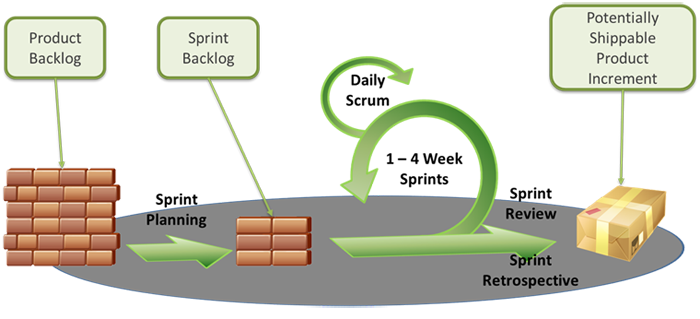
\includegraphics[scale=0.45]{images/ch_04/scrum_overview.png}
	  \end{center} 
	  \caption{\textit{Overview of the Scrum Process}}  
	  \label{fig:ScrumOverview}
  	\end{figure}


		\subsection{The Scrum Team}
		The \emph{Scrum Team} is composed of a \emph{Product Owner}, the \emph{Development Team}, and a \emph{Scrum Master}.
		These figures have different roles but all of them have to reach the same goal, deliver an increment part of usable product at constant time intervals (see \ref{Sprint Planning}). Scrum Teams are self-organizing and cross-functional. Self-organization gives the members the possibility to choose how best to accomplish their work, without being directed by others outside the team. Cross-functionality gives the team all the competencies needed to accomplish the work without depending on others not part of the team. The delivery of the products is iterative and incremental. This fact guarantees a constant feedback on the correctness of the job and ensures that a potentially useful version of the working product is always available ~\cite{scrumEnglishGuide}.

			\begin{figure}[h]
			  \begin{center} 
				%immagine senza copywright  :)
			    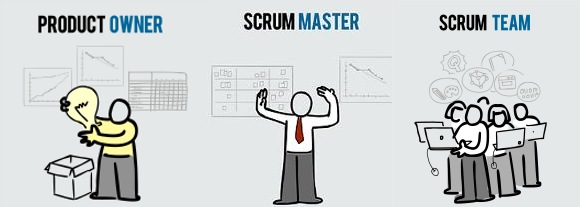
\includegraphics[scale=0.75]{images/ch_04/scrum_team_final.jpg}
			  \end{center} 
			  \caption{\textit{The Scrum Team}}  
			  \label{fig:ScrumTeam}
		  	\end{figure}
			


			\subsubsection{Product Owner}
			The \emph{Product Owner} is the person who represents the stakeholders of the job. The Product Owner can represent the will of a committee but must be one person. His or her role is to define the requirements that the new versions of the product must have, give them the priorities, explain them to the team in detail and is responsible for the performance of the team. These requirements are called \emph{Backlog Items} and are included in the \emph{Product Backlog}. This document is described in more details in the \ref{Artifacts} section ~\cite{scrumEnglishGuide}.

			\subsubsection{Development Team}
			The \emph{Development Team} consists of professionals who have to add the new functionalities to the product. The team are usually composed of three to nine members. One team must be self-organizing, this means that only the members can decide the step by step tasks to be accomplished in order to add the functionalities to the product. Every team is also cross-functional, i.e. is composed by people who have different skills. In this way it can be autonomous and it does not have to depend on other people outside the team to accomplish its job. More the Development Team's synergy is, more optimized its overall efficiency and effectiveness are ~\cite{scrumEnglishGuide}.
 
			\subsubsection{Scrum Master}
			The \emph{Scrum Master} has the role to verify that Scrum is understood and put in place. He or she does this checking that everyone in the team follows Scrum theory, practices, and rules. 
			The Scrum Master is the enforcer of the rules and interacts with all the people inside and outside the Scrum Team in order to teach which interactions are useful and which are not.
			On one side, he helps the Product Owner finding techniques for managing the \emph{Product Backlog}, teaching him how to communicate in clear way with the Development Team and in understanding and practicing agility. On the other side, he coaches the Development Team in self-organization and cross-functionality, he protects it from unhelpful interruptions and keeps it focused on the tasks. 
			For this, often this role is referred as a servant-leader for the Scrum Team ~\cite{scrumEnglishGuide}.


		\subsection{Events}
			Prefixed meetings in Scrum have the purpose to create regularity and hence to minimize the need for meetings not defined in Scrum, which can distract the members of the team from their tasks. In this events, different roles in the Scrum Team can interact with regularity, without the need for continuous interruptions. All the events are time-boxed, i.e. every event has a maximum duration. This ensures that only the appropriate amount of time is spent planning without waste of it ~\cite{scrumEnglishGuide}.   

			\begin{figure}[h]
			  \begin{center} 
				%immagine senza copywright  :)
			    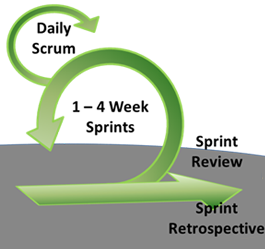
\includegraphics[scale=0.8]{images/ch_04/scrum_events.png}
			  \end{center} 
			  \caption{\textit{The Scrum Events}}  
			  \label{fig:ScrumEvents}
		  	\end{figure}
			


			
			\subsubsection{Sprint}
			The \emph{Sprint} is the primary unit of development in Scrum. It is a time-box with a fixed in advance duration. The duration can last from one week to one month. During this period of time the team creates finished portions of a product ~\cite{scrumEnglishGuide}. 
	
			Each Sprint is preceded by a \emph{Sprint Planning Meeting}, where the Scrum Team defines the tasks for the Sprint and gives an estimation for the Sprint goal. It ends with the \emph{Sprint Review Meeting} and \emph{Sprint Retrospective Meeting}, where the Scrum Team respectively reviews the progress and analyses the mistakes in the Scrum method and proposes solutions in order to avoid it in the next sprint. All these events will be described with more details in the next sections ~\cite{scrumEnglishGuide}.  


			\subsubsection{Sprint Planning Meeting}
			The \emph{Sprint Planning Meeting} is a meeting at which all the member of the Scrum Team participate. It precedes every Sprint. In this meeting the team decides which feature add to the product by the end of the Sprint ~\cite{scrumEnglishGuide}.

			At first the Product Owner informs the team of the features that he wants to be completely added to the product. Every feature is an item in the \emph{product backlog}. You can find a detailed description of this artifact in the section \ref{Product Backlog}. Then, the Development Team estimates how long it takes to add every new feature to the product and, consequently, how many of them will be added by the end of the Sprint. Often this part of the meeting is signed by a clarification about the requirements between the Product Owner and the Development Team that leads to new time estimation for each goal. The goals are split into tasks, each of which takes no more than one day to be accomplished by the development team. Every task and the plan for delivery them are collected in the \emph{Sprint Backlog}. A detailed description of this document can be found in the section \ref{Sprint Backlog} ~\cite{scrumEnglishGuide}.

			Every Sprint must have a \emph{Sprint Goal}. The Sprint Goal acts like a sort of motivation which reminds the Development Team during the whole sprint which is in a wider context the goal of their activities. For this the sprint goals should not be changed during the sprint ~\cite{scrumEnglishGuide}.
		
			\subsubsection{Daily Scrum}
			The \emph{Daily Scrum} is a fifteen minutes event for the Development Team, that allows the team to synchronize the work and plan the next day activities. This purpose is achieved analyzing the work done in the last day and forecasting the work for the next one. 
			During the meeting, each Development Team member explains what he did since the last meeting, what he is going to do before the next meeting and the problems he has to front.
			The meeting has the purpose to evaluate the progress towards the Sprint Goal and to analyze the trend of the progress in comparison with the Sprint Backlog ~\cite{scrumEnglishGuide}. 

			\subsubsection{Sprint Review}
			The \emph{Sprint Review} is a time-boxed meeting which closes every Sprint. In this meeting the increment of the work is analyzed and, if needed, the Product Backlog is updated. 
			During the meeting, the Product Owner analyzes what has been completed and what has not been completed. The Development Team describes the problem it encountered, how it solved them and shows the new functionalities added to the product. Then the whole team discusses of new opportunities and, more generally, collaborates on what to do next, updating consequently the Product Backlog ~\cite{scrumEnglishGuide}.			

			\subsubsection{Sprint Retrospective}
			The \emph{Sprint Retrospective} is a time-boxed meeting which is fixed after ever Sprint Review. It is an opportunity for the Scrum Team to analyze its scrum implementation and create a plan for the improvements of the next Sprint. 
			During the meeting the focus is set on people, relationships, process and tools. The most important successes are shown and a plan for implementing potential improvements is created. 
			The purpose of this meeting is to make the implementation of the method more effective optimizing the development process and introducing techniques that make the method more productive and enjoyable ~\cite{scrumEnglishGuide}. 

		
		\subsection{Artifacts}
			Scrum's \emph{artifacts} represent the work in many different ways. The basic artifacts required by the framework are the Product Backlog and the Sprint Backlog.

			\subsubsection{Product Backlog}
			The \emph{Product Backlog} is an artifact which contains the list of the requirement for a product. The elements of the list, called \emph{Backlog Items}, are sorted by priority. 

			Every Item must have a name, a description, an estimate and a priority. For each Item, the Product Owner, representing the stakeholder will, sets the priority and	 the Development Team defines the estimate.

			The Product Backlog is dynamic. The earliest versions of it only contain the initially and best understood requirements of the product. Then, as long as the product evolves and new requirements are introduced, it is continuously updated. In this way, it always contains all the features, enhancements and fixes that must be added in the future at the product. 

			As the higher ordered Items are more important than lower ordered ones, they are clearer and more detailed. The team makes more precise estimates basing on the greater clarity and increased detail. The lower the order of the items, the less detailed are the description and the time estimation.
			
			The activity of adding detail, estimates, and order to the items in the Product Backlog is called \emph{grooming}. The Scrum Team decides how and when doing it. Anyway the grooming activity must not consume more than the 10\% of the capacity of the team.
		

			\subsubsection{Sprint Backlog}
			The \emph{Sprint Backlog} contains the \emph{Product Backlog Items} selected for the current Sprint and a plan for completing all the modification to the product and realizing the Sprint Goal. 
			The Sprint Backlog is a forecast about which functionalities should be added to the product by the end of the Sprint and, at the same time, monitors the state of the work during every day of the Sprint ~\cite{scrumEnglishGuide}.
			
			\begin{figure}[h]
			  \begin{center} 
			    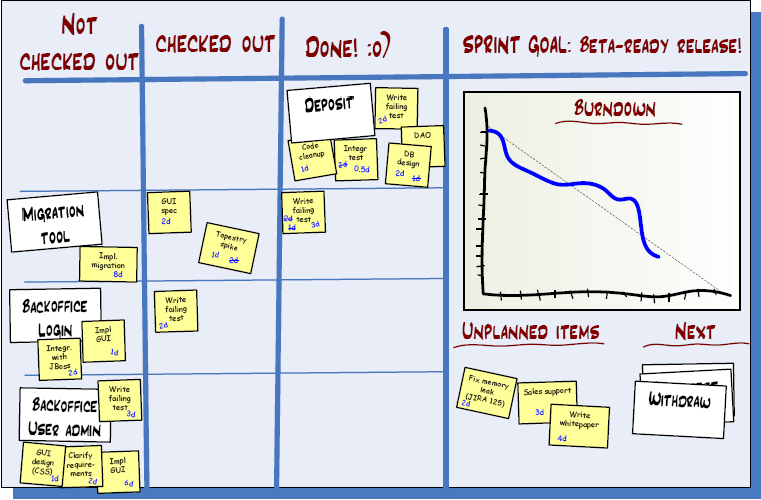
\includegraphics[scale=0.65]{images/ch_04/task_board_and_chart.png}
			  \end{center} 
			  \caption{\textit{Sprint Backlog and Burn Down Chart}}  
			  \label{fig:SprintBacklog}
		  	\end{figure}

			The level of detail of the work is such that it can be measured during the \emph{Daily Scrum}. Usually every Product Backlog Item is split into tasks, each of which must be accomplished in not more than than sixteen hours of work. The tasks are never assigned; rather, every member of the team takes charge of one of it during the daily scrum, according to the set priority and the Development Team member skills.
	
			The Sprint Backlog is updated every day during the \emph{Daily Scrum}. If some new work emerges to be necessary in order to complete some requirements, the Development Team adds it to the Sprint Backlog. If there are some elements which are deemed unnecessary, they are removed.

			The state of the ongoing activities can be monitored by a \emph{Burn Down Chart}, which measures the number of completed tasks per day and compares it with an ideal trend, which represents the estimates of the tasks. This chart allows to analyze the accuracy of the estimates and to have a visual representation of the ongoing work ~\cite{scrumEnglishGuide}.

					
			
	
	
	% TODO 
	\section{The Adopted Development Process}
		%Cose che voglio dire:
		1) Processo di sviluppo incementale e iterativo
		2) No pair programmin nè test driven development  (dirlo ? )
		3) Sviluppo agile
		4) Come abbiamo usato noi SCRUM
			-) sprint: 2 settimane
			-) non c'era un committente ma c'era il project manager
			-) 1 team

\begin{comment}
	\section{SCRUM}

	\section{Working Instruments}
	In addition to ACT-R and OpenCV, many other tools have been used. Here follows a list of the most important ones.
		\begin{itemize}
		\item \textbf{Eclipse IDE for C/C++ Developers} as \textit{integrated development environment} \footnote{More informations at \url{www.eclipse.org}};
		\item \textbf{Cute} as \textit{unit testing framework} \footnote{More informations at \url{http://cute-test.com}};
		\item \textbf{Mylyn} as \textit{task and application lifecycle management} \footnote{More informations at \url{www.eclipse.org/mylyn}};
		\item \textbf{Trac} as \textit{bug tracking system} \footnote{More informations at \url{trac.edgewall.org}};
		\item \textbf{Git} as \textit{version control system} \footnote{More informations at \url{git-scm.com}}; 
		\item \textbf{Dia} and \textbf{cpp2dia} to create UML diagrams \footnote{More informations at \url{dia-installer.de} and at \url{cpp2dia.sourceforge.net}};
		\item \textbf{ZBar} to read QR codes \footnote{More informations at \url{zbar.sourceforge.net}}.
		%%It can be useful for drawing a large variety of diagrams, in particular UML diagrams, network maps and flowcharts. 
		\end{itemize}
\end{comment}
